\documentclass[a4paper,openright,12pt]{report}
%Modificamos el tipo de papel a A4 y el tamaño de la fuente.
%El tipo de documento a sido modificado a tipo informe o reporte.

\usepackage{fullpage}
\usepackage{listings}
\usepackage{graphicx}

\begin{document}

\title{Plan de tesis}
\author{Villanueva Portella, Jhon Gesell}
\date{25/06/2018}
\maketitle

\section{Introducci\'on}
%	\begin{itemize}
%	\item Importancia
%	\item Antecedentes
%	\item Justificaci\'on del m\'etodo utilizado
%	\item Valor agregado de nuestra propuesta	
%	\end{itemize}
Un paquete hidro-sedimentario ayuda a la toma de mejores decisiones en la gesti\'on de los recursos h\'idricos consolidando una base de datos que permita recopilar a lo largo de los años los datos de hidr\'aulica y de sedimentos. Esta base ayuda a poder analizar el comportamiento de los rios, determinar las \'epocas de m\'aximas crecidas y secas.

Contar con una base igualmente permite tener un mejor acceso para un mayor p\'ublico cient\'ifico y t\'ecnico.

Una de las ventajas de tener una herramienta con paquetes libres es el acceso, la continua actualizaci\'on y evitar la pirateria.



El paquete que se desea proponer estar\'a alojado en una plataforma web que permita colocar los datos en una nube, sin embargo el primer paso es hacer esto posible en un localhost que  brinde posibilidades de acceso desde centros de estudio, centros de investigaci\'on o incluso para el sector privado; nuestra propuesta pretende beneficiar a todos ellos con este motivo se pone bajo la licencia GPL ( General Public License).
\section{Objetivos}
	\subsection{Ojetivo General}
	\begin{itemize}
	\item Crear un software hidrosedimentario con interfaz gr\'afica de usuario.
	\item Brindar un producto que ayude a los cient\'ificos e ingenieros que trabajan con flu\'idos geof\'isicos.
	\item Entregar un producto open-source para la comunidad cient\'ifica internacional.
	\end{itemize}
	\subsection{Objetivo Espec\'ifico}
	\begin{itemize}
	\item Crear una lectura de archivos de caudales.
	\item Crear un formulario para insertar los datos de las muestras se sedimentos.
	\item Crear una base de datos.
	\item Gr\'aficar la sección del r\'io para visualizar las cotas de fondo y los valores de sedimentos en suspensi\'on.
	\end{itemize}

\section{Hip\'otesis}
	El software debe ser calibrado con el modelo HidroMESAD y ofrecer valores cercanos al $5\%$ de este.

\section{Materiales y m\'etodos}
\begin{enumerate}
\item Materiales
	\begin{enumerate}
	\item Archivos de secci\'on datos de batimetria (profundidad y distancia referidas a una orilla), tambi\'en el de la velociad en la sección: \\
	Los datos son importados desde el ordenador del usuario.
	\item Datos ingresados por el usuario: \\
	Es insertar en el software la tabla de muestras procesadas en laboratorio.
	\item Framework de desarrollo de aplicaciones con interfaz gr\'afica de usuario: \\
	Utilizamos PyQt5, entorno que nos permite trabajar con el lenguaje Python haciendo uso de multiples clases.
	\item Lenguaje de programaci\'on Python 2.x y 3.x: \\
	Es un lenguaje open-source multiplataforma y multiprop\'osito que viene creciendo en diferentes campos, hoy muy usado en el campo cient\'ifico, tiene una gran comunidad en todo el mundo, tiene una sint\'axis f\'acil y limpia.
	\item SQLite: \\
	Es un facilitador de base de datos liviano y robusto multiplataforma teniendo alcance hasta para aplicaciones móbiles.
	\item Scrum: \\
	Es un marco metodol\'ogico \'agil hoy muy usado en el desarrollo de software y tambi\'en va calando en otros rubros, se trata de hacer iteraciones (pivotear), trabajar a partir de un prototipo funcional y a partir de esto seguir avanzando, en caso pare el proyecto siempre haya algo que mostrar.
	\item VIM: \\
	Vim es un editor de texto plano mejorado que nos permite navegar desde la terminal del sistema operativo GNU/Linux o Windows.
	\end{enumerate}
\item M\'etodos
	\begin{enumerate}
	\item Lectura de archivos brindados por el usuario.
	\item Insertar datos por el usuario.
	\item Almacenamiento en la base de datos.
	\item Generaci\'on de una matr\'iz.
	\item Interpolaci\'on de puntos.
	\item Gr\'afica de la secci\'on del r\'io.
	\item Gr\'afica de las celdas de aforo.
	\item C\'alculo del caudal.
	\end{enumerate}
\end{enumerate}
\section{Resultados esperados}

\begin{enumerate}

\item Viesta preliminar de la interfaz gr\'afica de usuario \\
Para ello vea a la Figura~\ref{fig:Vista_preliminar_de_HyDro-Desktop}

\begin{figure}
  \centering
    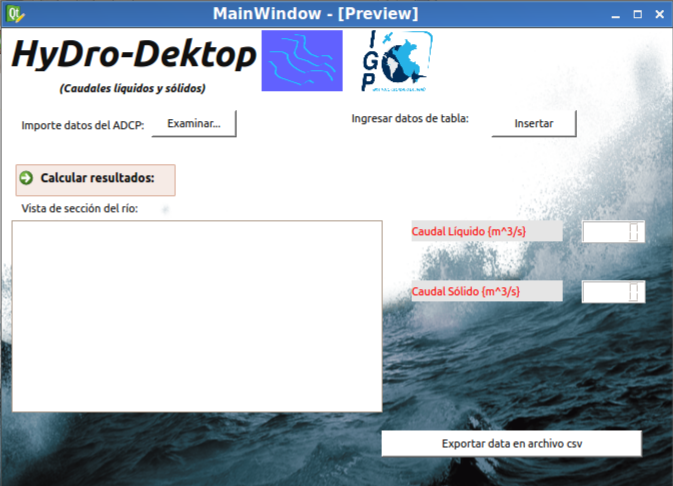
\includegraphics[width=0.7\textwidth]{screet_preview}
  \caption{Vista constru\'ida con Qt Designer}
  \label{fig:Vista_preliminar_de_HyDro-Desktop}
\end{figure}

\item Base de datos
Se ha elaborado unos scripts que permiten crear la tabla; llenar, actualizar y eliminar los registros que constituyen la base de datos. Todo esto se logró desde el lenguaje Python2.x, los c\'odigos se visualizan en los Anexos 01, 02 y 03 respectivamente.

Para ello vea a la Figura~\ref{fig:Vista_archivo_database_sediments}



\begin{figure}
  \centering
    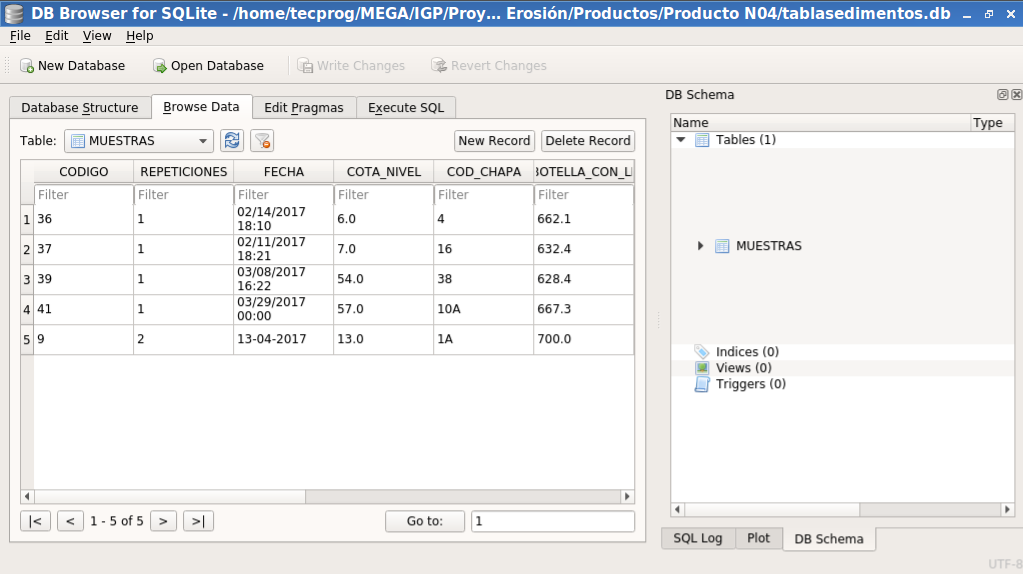
\includegraphics[width=0.7\textwidth]{screet_database}
  \caption{Tabla ingresada por el usuario desde la terminal}
  \label{fig:Vista_archivo_database_sediments}
\end{figure}


\end{enumerate}

\section{Cronograma}

\begin{center}

\begin{tabular}{|c|c|c|c|c|c|c|c|}
\hline
Meses & Junio & Julio & Agosto & Septiembre & Octubre & Noviembre & Diciembre\\ \hline
R.I. & x &  - & - & - & - & - & - \\ \hline
L.B. & x &  x & - & - & - & - & - \\ \hline
C.B.D. & x &  - & - & - & - & - & - \\ \hline
C.F. & x &  - & - & - & - & - & - \\ \hline
I.F.B.D. & - & x & - & - & - & - & - \\ \hline
I.R. & - &  - & x & x & - & - & - \\ \hline
A.M. & - &  - & - & - & x & - & - \\ \hline
C.M. & - &  - & - & - & - & x & - \\ \hline
M.U. & - &  - & - & - & - & - & x \\ \hline
\end{tabular}

\end{center}

\begin{itemize}
\item Leyenda:
	\begin{itemize}
	\item R.I.: Recolecci\'on de informaci\'on.
	\item L.B.: Lectura de la bibliograf\'ia.
	\item C.B.D.:Creaci\'on de la base de datos.
	\item C.F.: Creaci\'on del formulario.
	\item I.F.B.D.: Implementaci\'on funcional de la base de datos.
	\item I.R.: Impresi\'on de resultados en la GUI.
	\item A.M.: Ajustes del modelo.
	\item C.M.: Correcci\'on del modelo.
	\item M.U.: Manual de usuario.
	\end{itemize}
\end{itemize}

\section{Discusiones}

\section{Conclusiones}

\section{Bibliograf\'ia}
\begin{itemize}
	\item Gonz\'ales, R. (s.f.). \textit{Python para todos}. Recuperado de: \textbf{http://mundogeek.net/tutorial-python}
	\item Coutinho, N. (2016). \textit{Introducci\'on a la programaci\'on con Python: Algoritmos y l\'ogica de programaci\'on para principiantes}, Brasil: Novatec Editora Ltda.
	\item Harwani, B. (2012). \textit{Introduction to Python Programming and Developing GUI Applications with PyQT}, Estados Unidos: Course Technology PTR .
\end{itemize}

\section{Anexos}
\subsection{Base de datos}
\begin{enumerate}
\item Creaci\'on de la tabla. \\
\textit{CrearTablaSedimentos.py}
\begin{lstlisting}
#!/usr/bin/python
# -*- coding: cp1251 -*-

# Crear base de datos y tabla con sqlite3
# 20/06/2018

__autor__ = u"Jhon Gesell"

import sqlite3

conexion = sqlite3.connect('tablasedimentos.db')
cursor = conexion.cursor()

#Crear tabla
cursor.execute('''CREATE TABLE MUESTRAS
                (CODIGO TEXT NOT NULL,
                 REPETICIONES TEXT NOT NULL,
                 FECHA TEXT NOT NULL,
                 COTA_NIVEL REAL NOT NULL,
                 COD_CHAPA TEXT NOT NULL,
                 PESO_BOTELLA_CON_LIQUIDO REAL NOT NULL,
                 PESO_BOTELLA REAL NOT NULL,
                 VOLUMEN REAL NOT NULL,
                 FINOS_PESO_INICIAL_FILTRO REAL NOT NULL,
                 FINOS_PESO_FINAL_FILTRO REAL NOT NULL,
                 GRUESOS_PESO_INICIAL_FILTRO REAL NOT NULL,
                 GRUESOS_PESO_FINAL_FILTRO REAL NOT NULL,
                 ESTACION TEXT NOT NULL)''')
conexion.close()

\end{lstlisting}

\item Insersi\'on de registros en los campos. \\
\textit{datossedimetos.py}
\begin{lstlisting}
#!/usr/bin/python
# -*- coding: cp1252 -*-

# Insertar datos de una tabla con sqlite3
# 21/06/2018

__autor__ = u"Jhon Gesell"

import sqlite3

codigo = raw_input("Codigo: ")
repeticiones = raw_input("Repeticiones: ")
fecha = raw_input("Fecha: ")
cota_nivel = raw_input("Cota nivel: ")
cod_chapa = raw_input("Codigo de botella: ")
peso_botella_con_liquido = raw_input("Peso botella con liquido:
")
peso_botella = raw_input("Peso botella: ")
volumen = raw_input("Volumen: ")
finos_peso_inicial_filtro = raw_input("Peso inicial filtro fino:
")
finos_peso_final_filtro = raw_input("Peso final filtro fino:
")
gruesos_peso_inicial_filtro = raw_input("Peso inicial filtro
grueso:
")
gruesos_peso_final_filtro = raw_input("Peso final filtro grueso:
")
estacion = raw_input("Estacion: ")

conexion = sqlite3.connect('tablasedimentos.db')
cursor = conexion.cursor()

#Insertar datos en la tabla
cursor.execute('''INSERT INTO MUESTRAS(CODIGO, REPETICIONES,
FECHA, COTA_NIVEL, COD_CHAPA, PESO_BOTELLA_CON_LIQUIDO,
PESO_BOTELLA, VOLUMEN, FINOS_PESO_INICIAL_FILTRO,
FINOS_PESO_FINAL_FILTRO, GRUESOS_PESO_INICIAL_FILTRO, 
GRUESOS_PESO_FINAL_FILTRO, ESTACION)
                VALUES ('%s', '%s', '%s', '%s', '%s',
                '%s', '%s', '%s', '%s', '%s', '%s', '%s', '%s')
                ''' %(codigo, repeticiones, fecha, cota_nivel,
                cod_chapa, peso_botella_con_liquido,
                peso_botella,
                volumen, finos_peso_inicial_filtro,
                finos_peso_final_filtro,
                gruesos_peso_inicial_filtro,
                gruesos_peso_final_filtro, estacion))

conexion.commit()
conexion.close()
\end{lstlisting}

\item Actualizaci\'on de registros en los campos. \\
\textit{ActualizarSedimentos.py}
\begin{lstlisting}
#!/usr/bin/python
#-*- coding: cp1252 -*-

# Actualizar datos en una tabla con sqlite3
# 23/06/2018

__autor__ = u"Jhon Gesell"

import sqlite3

#codigo = raw_input("Codigo: ")
#repeticiones = raw_input("Repeticiones: ")
fecha = raw_input("Fecha: ")
#cota_nivel = raw_input("Cota nivel: ")
cod_chapa = raw_input("Codigo de botella: ")
#peso_botella_con_liquido = raw_input("Peso botella con liquido:
")
#peso_botella = raw_input("Peso botella: ")
volumen = raw_input("Volumen: ")
#finos_peso_inicial_filtro = raw_input("Peso inicial filtro fino:
")
#finos_peso_final_filtro = raw_input("Peso final filtro fino:
")
#gruesos_peso_inicial_filtro = raw_input("Peso inicial filtro
grueso: ")
#gruesos_peso_final_filtro = raw_input("Peso final filtro grueso:
")
#estacion = raw_input("Estacion: ")

conexion = sqlite3.connect('tablasedimentos.db')
cursor = conexion.cursor()

#Actualizar datos en la tabla
cursor.execute("UPDATE MUESTRAS SET VOLUMEN=:volumen
WHERE FECHA=:fecha and COD_CHAPA=:cod_chapa",
                {"volumen": volumen, "fecha": fecha,
                "cod_chapa": cod_chapa})

conexion.commit()
\end{lstlisting}

\item Eliminaci\'on de registros por campos. \\
\textit{vaciartablasedimentos.py}
\begin{lstlisting}
#!/usr/bin/python
#-*- coding: cp1252 -*-

# Borrar datos en una tabla con sqlite3

__autor__ = u"Jhon Gesell"

import sqlite3

codigo = raw_input("Codigo: ")
#repeticiones = raw_input("Repeticiones: ")
#fecha = raw_input("Fecha: ")
#cota_nivel = raw_input("Cota nivel: ")
#cod_chapa = raw_input("Codigo de botella: ")
#peso_botella_con_liquido = raw_input("Peso botella con liquido:
")
#peso_botella = raw_input("Peso botella: ")
#volumen = raw_input("Volumen: ")
#finos_peso_inicial_filtro = raw_input("Peso inicial filtro fino:
")
#finos_peso_final_filtro = raw_input("Peso final filtro fino:
")
#gruesos_peso_inicial_filtro = raw_input("Peso inicial filtro
grueso: ")
#gruesos_peso_final_filtro = raw_input("Peso final filtro
grueso: ")
#estacion = raw_input("Estacion: ")

conexion = sqlite3.connect('tablasedimentos.db')
cursor = conexion.cursor()

#Eliminar datos en la tabla

cursor.execute("DELETE FROM MUESTRAS WHERE CODIGO = %s" %codigo)
conexion.commit()

conexion.close()
\end{lstlisting}


\end{enumerate}

\end{document}